\subsubsection{终端命令解析}

\begin{longtable}{|r|l|l|}
	\caption{当前支持的命令} 
\label{tab:supported-commands} \\

\hline
\textbf{命令名称} & \textbf{命令格式} & \textbf{命令行为} \\ \hline
CUU & ESC [ Pn\footnote{Pn表示数值参数,可以省略} A & 光标上移\\ \hline
CUD & ESC [ Pn B & 光标下移\\ \hline
CUF & ESC [ Pn C & 光标前进\\ \hline
CUB & ESC [ Pn D & 光标后退\\ \hline
CNL & ESC [ Pn E & 光标下移到行首\\ \hline
CPL & ESC [ Pn F & 光标上移到行首\\ \hline
CHA & ESC [ Pn G & 光标水平移动\\ \hline
VPA & ESC [ Pn d & 光标垂直移动\\ \hline
CUP/HVP & ESC [ Pn; Pn f/H & 设置光标位置\\ \hline \hline

REP & ESC [ Pn b & 重复上一个输入的字符 \\ \hline
DL & ESC [ Pn M &删除行 \\ \hline
IL & ESC [ Pn L &插入行 \\ \hline
ED &ESC [ Pn J &删除部分显示的文本 \\ \hline
EL &ESC [ Pn K &删除部分当前行文本 \\ \hline
ECH & ESC [ Pn X &清除部分字符 \\ \hline
DCH & ESC [ Pn P &删除部分字符 \\ \hline
ICH & ESC [ Pn @ &插入空白字符 \\ \hline \hline

SETDEC & ESC [? Ps\footnote{Ps表示由分号分隔的个数不定的数值参数列} h & 设置DEC模式 \\ \hline
RESETDEC & ESC [? Ps l & 清除DEC模式 \\ \hline
SETMODE &ESC [ Ps h & 设置模式 \\ \hline
RESETMODE & ESC [ Ps l &清除模式 \\ \hline \hline

NEL & ESC E &新行 \\ \hline
RI & ESC M & 回到上一行 \\ \hline
IND & ESC D &转到下一行 \\ \hline
DECSC & ESC 7& 保存光标状态 \\ \hline
DECRC &ESC 8& 恢复光标状态 \\ \hline \hline

SU & ESC [ Pn S &向上滚动 \\ \hline
SD & ESC [ Pn T &向下滚动 \\ \hline
DECSTBM & ESC [ Pn; Pn r &设置滚动区域 \\ \hline \hline

SS2 & ESC N&设置字符集 \\ \hline
SS3 & ESC O&设置字符集 \\ \hline
SCS0 & ESC ( A/B/0/1/2 & 设置字符集 \\ \hline
SCS1 & ESC ) A/B/0/1/2 &设置字符集 \\ \hline \hline

SGR & ESC [ Ps m &设置颜色等字符信息 \\ \hline
\end{longtable}
\begin{figure}[htbp]
\centerline{
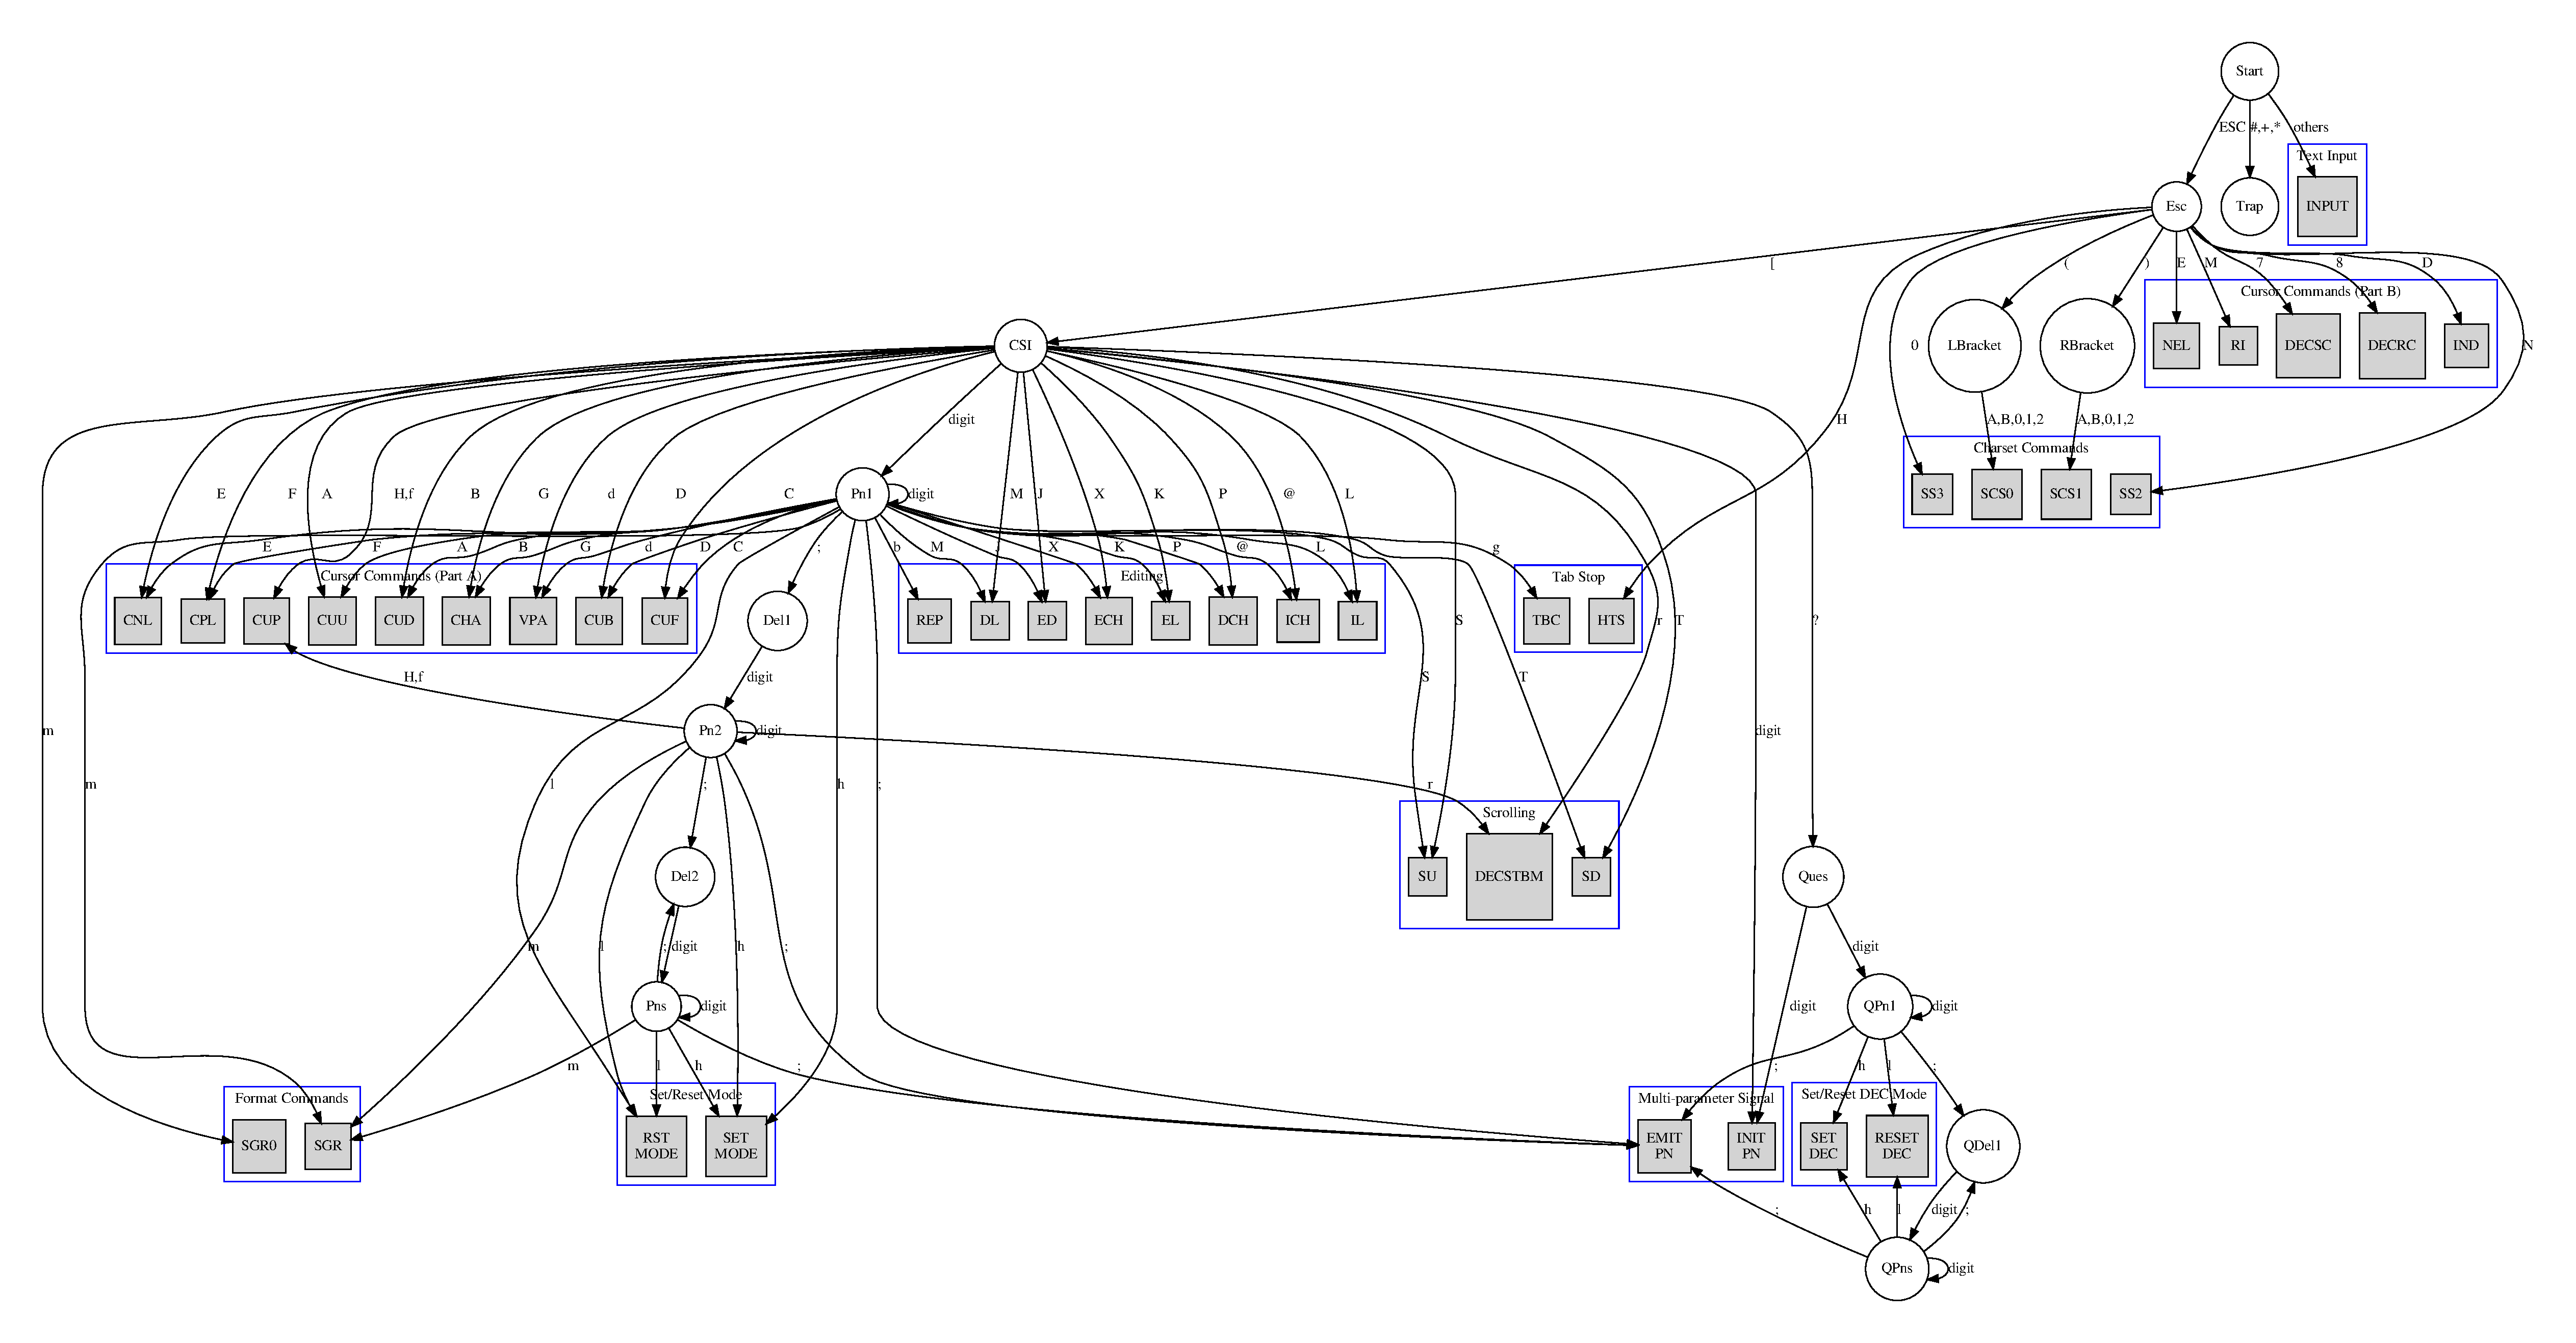
\includegraphics[width=0.95\paperwidth]{command_parser.pdf}
}
\label{fig:command_parser}
\caption{命令解析状态图,圆形节点为状态,方形为命令。}
\end{figure}
